\documentclass[border=2pt]{standalone}
\usepackage{amsmath}
\usepackage{amssymb}
\usepackage{fontspec}
\setsansfont{Arial}
\renewcommand{\familydefault}{\sfdefault}
\usepackage{tikz}
\usetikzlibrary{arrows.meta,positioning,calc,fit,backgrounds,shapes.geometric}
\definecolor{titlegray}{HTML}{5F6B78}
\definecolor{ent}{HTML}{7B8794}
\definecolor{fo}{HTML}{5AA9C4}
\definecolor{ho}{HTML}{2E6B86}
\definecolor{inf}{HTML}{D98A3D}
\definecolor{vio}{HTML}{9B86C4}
\definecolor{smac}{HTML}{2E8AA6}
\definecolor{kgc}{HTML}{E7B15A}
\definecolor{kgc2}{HTML}{D39A3E}
\definecolor{g1}{HTML}{C7CCD1}
\definecolor{g2}{HTML}{A7AFB6}
\definecolor{g3}{HTML}{7E8893}
\definecolor{g4}{HTML}{5B6670}
\definecolor{fillteal}{HTML}{E3EEF2}
\definecolor{fillamber}{HTML}{FBF0E2}
\definecolor{fillgrey}{HTML}{F1F3F5}
\definecolor{ribA}{HTML}{CFE3D6}
\definecolor{ribB}{HTML}{CFE0E8}
\definecolor{ribC}{HTML}{D7D2E8}
\definecolor{ribD}{HTML}{F3DDD0}
\definecolor{inkmid}{HTML}{3D4751}
\begin{document}
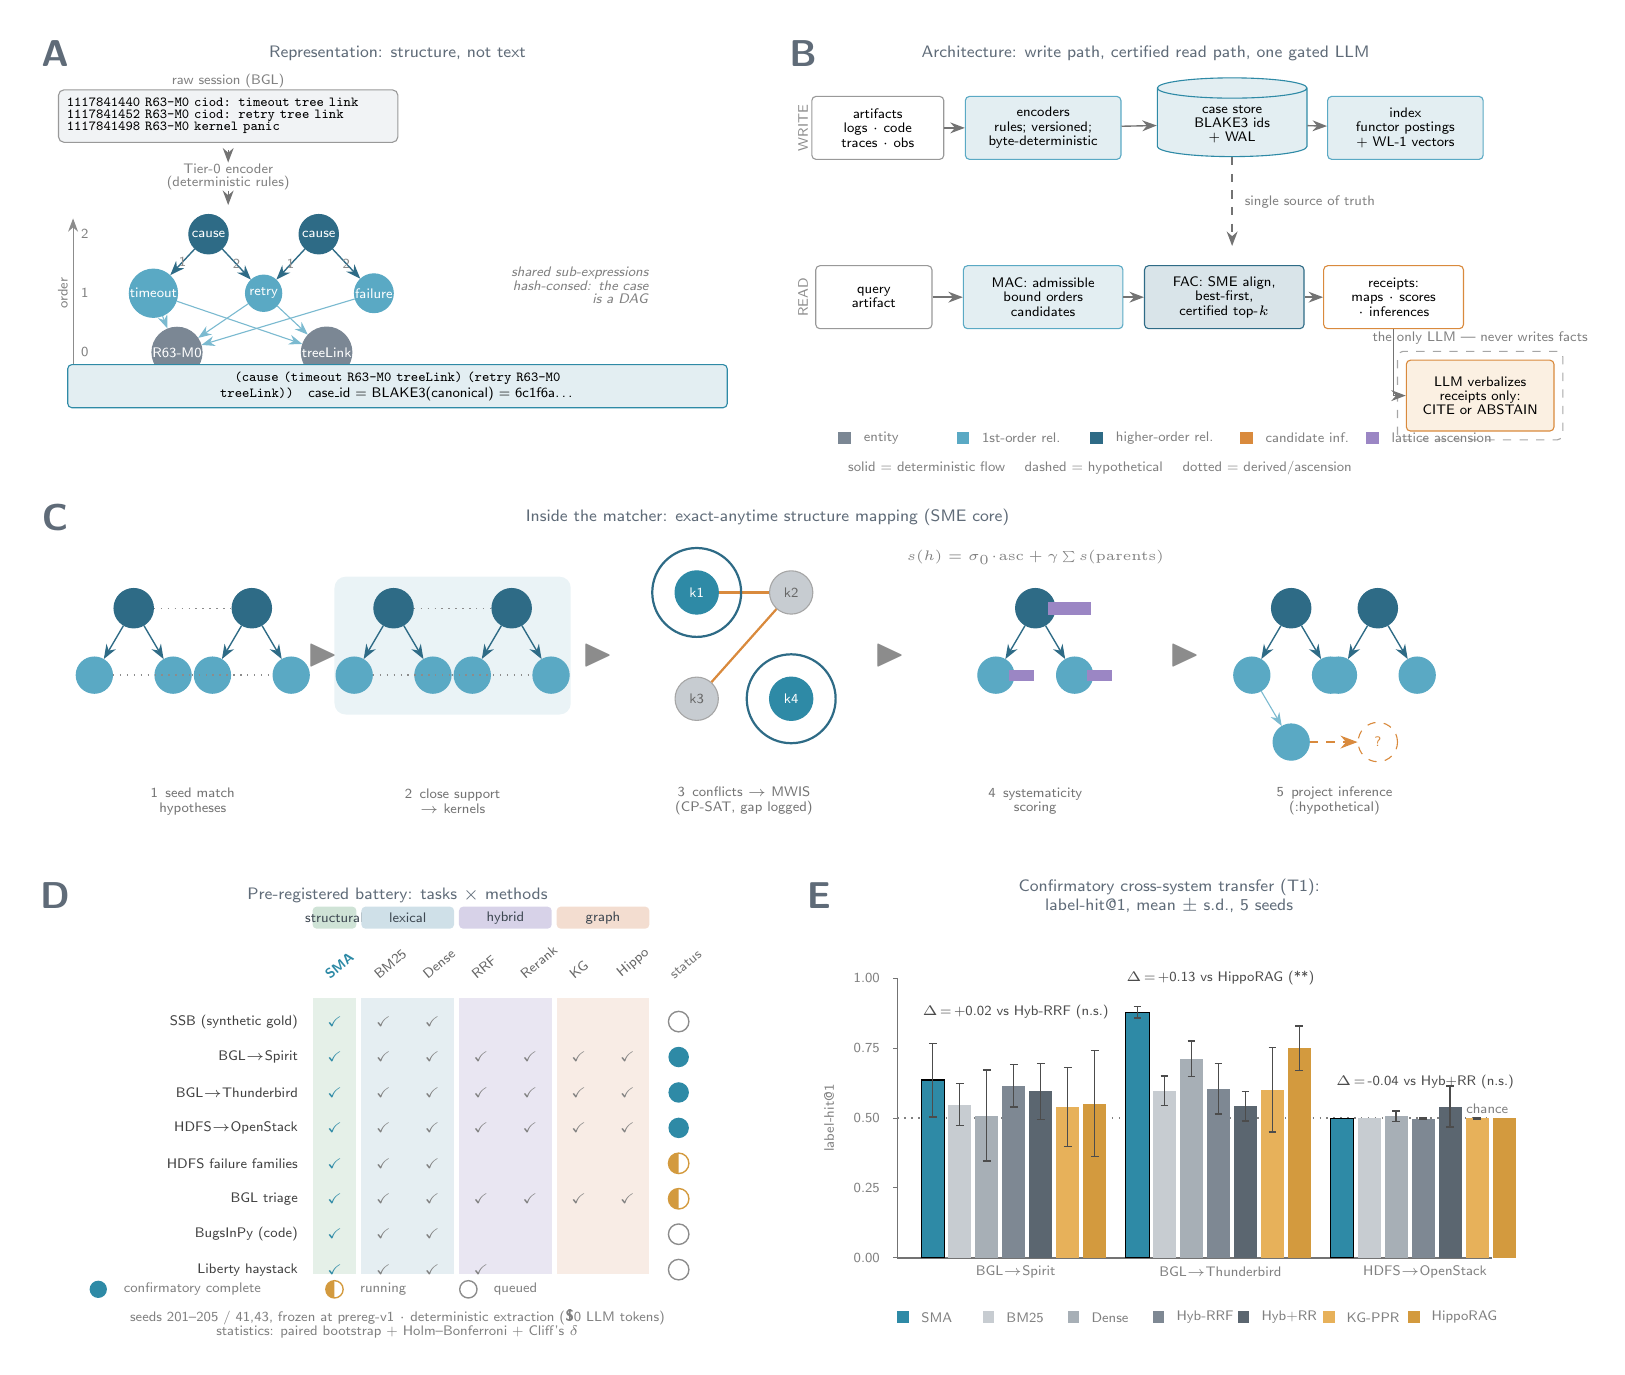
\begin{tikzpicture}[
  font=\sffamily,
  >=Stealth,
  ptitle/.style={font=\sffamily\bfseries\small, color=titlegray},
  pletter/.style={font=\sffamily\bfseries, color=titlegray, scale=1.35},
  ttl/.style={font=\sffamily\fontsize{6}{7}\selectfont, color=titlegray, align=center},
  sub/.style={font=\sffamily\fontsize{4.6}{5.4}\selectfont, color=black!55, align=center},
  micro/.style={font=\sffamily\fontsize{4}{4.8}\selectfont, color=black!50, align=center},
  enode/.style={circle, draw=ent, fill=ent, text=white, font=\sffamily\fontsize{4}{4.6}\selectfont, inner sep=0pt, minimum size=4.2mm, align=center},
  fnode/.style={circle, draw=fo, fill=fo, text=white, font=\sffamily\fontsize{4}{4.6}\selectfont, inner sep=0pt, minimum size=4.6mm, align=center},
  hnode/.style={circle, draw=ho, fill=ho, text=white, font=\sffamily\fontsize{4}{4.6}\selectfont, inner sep=0pt, minimum size=5mm, align=center},
  pbox/.style={rounded corners=1.5pt, draw, align=center, inner sep=2.5pt, font=\sffamily\fontsize{4.4}{5.2}\selectfont},
  flowarr/.style={->, line width=0.5pt, color=black!55},
  horel/.style={->, line width=0.5pt, color=ho},
  forel/.style={->, line width=0.4pt, color=fo!80},
]
\begin{scope}[shift={(0,11.9)}]
\node[pletter] at (-0.05,4.35) {A};
\node[ttl] at (4.3,4.35) {Representation: structure, not text};
\node[draw=black!40, fill=fillgrey, rounded corners=2pt, align=left, inner sep=3pt, font=\ttfamily\fontsize{3.6}{4.4}\selectfont, text width=4.1cm] (log) at (2.15,3.55) {1117841440 R63-M0 ciod: timeout tree link\\1117841452 R63-M0 ciod: retry tree link\\1117841498 R63-M0 kernel panic};
\node[micro] at (2.15,4.0) {raw session (BGL)};
\node[micro, align=center] (enc) at (2.15,2.78) {Tier-0 encoder\\(deterministic rules)};
\draw[flowarr] (2.15,3.12) -- (2.15,2.96);
\draw[flowarr] (2.15,2.6) -- (2.15,2.42);
\draw[->, line width=0.4pt, color=black!45] (0.18,0.35) -- (0.18,2.25);
\node[micro, rotate=90] at (0.05,1.3) {order};
\node[micro] at (0.33,0.55) {0};
\node[micro] at (0.33,1.3) {1};
\node[micro] at (0.33,2.05) {2};
\node[enode] (e1) at (1.5,0.55) {R63-M0};
\node[enode] (e2) at (3.4,0.55) {treeLink};
\node[fnode] (f1) at (1.2,1.30) {timeout};
\node[fnode] (f2) at (2.6,1.30) {retry};
\node[fnode] (f3) at (4.0,1.30) {failure};
\node[hnode] (h1) at (1.9,2.05) {cause};
\node[hnode] (h2) at (3.3,2.05) {cause};
\draw[horel] (h1) -- (f1) node[midway, font=\sffamily\fontsize{3.2}{3.6}\selectfont, color=black!45, inner sep=1pt] {1};
\draw[horel] (h1) -- (f2) node[midway, font=\sffamily\fontsize{3.2}{3.6}\selectfont, color=black!45, inner sep=1pt] {2};
\draw[horel] (h2) -- (f2) node[midway, font=\sffamily\fontsize{3.2}{3.6}\selectfont, color=black!45, inner sep=1pt] {1};
\draw[horel] (h2) -- (f3) node[midway, font=\sffamily\fontsize{3.2}{3.6}\selectfont, color=black!45, inner sep=1pt] {2};
\draw[forel] (f1) -- (e1);
\draw[forel] (f1) -- (e2);
\draw[forel] (f2) -- (e1);
\draw[forel] (f2) -- (e2);
\draw[forel] (f3) -- (e1);
\node[micro, align=right, text width=2.6cm] at (6.2,1.4) {\textit{shared sub-expressions}\\\textit{hash-consed: the case}\\\textit{is a DAG}};
\node[pbox, draw=smac, fill=fillteal, text=black, font=\sffamily\fontsize{3.8}{4.6}\selectfont, text width=8.2cm, align=center] at (4.3,0.12) {\texttt{(cause (timeout R63-M0 treeLink) (retry R63-M0 treeLink))}\quad case\_id = BLAKE3(canonical) = 6c1f6a\ldots};
\end{scope}
\begin{scope}[shift={(9.5,11.9)}]
\node[pletter] at (-0.05,4.35) {B};
\node[ttl] at (4.3,4.35) {Architecture: write path, certified read path, one gated LLM};
\node[micro, rotate=90, color=black!45] at (-0.05,3.4) {WRITE};
\node[pbox, draw=black!40, fill=white, text width=1.5cm, minimum height=8mm] (art) at (0.9,3.4) {artifacts\\logs $\cdot$ code\\traces $\cdot$ obs};
\node[pbox, draw=fo, fill=fillteal, text width=1.8cm, minimum height=8mm] (enc2) at (3.0,3.4) {encoders\\rules; versioned;\\byte-deterministic};
\node[cylinder, shape border rotate=90, draw=smac, fill=fillteal, aspect=0.25, minimum width=1.9cm, minimum height=1.0cm, inner sep=1pt, font=\sffamily\fontsize{4.2}{5}\selectfont, align=center] (store) at (5.4,3.45) {case store\\BLAKE3 ids\\+ WAL};
\node[pbox, draw=fo, fill=fillteal, text width=1.8cm, minimum height=8mm] (idx) at (7.6,3.4) {index\\functor postings\\+ WL-1 vectors};
\draw[flowarr] (art) -- (enc2); \draw[flowarr] (enc2) -- (store); \draw[flowarr] (store) -- (idx);
\node[micro, rotate=90, color=black!45] at (-0.05,1.25) {READ};
\node[pbox, draw=black!40, fill=white, text width=1.3cm, minimum height=8mm] (q) at (0.85,1.25) {query\\artifact};
\node[pbox, draw=fo, fill=fillteal, text width=1.85cm, minimum height=8mm] (mac) at (3.0,1.25) {MAC: admissible\\bound orders\\candidates};
\node[pbox, draw=ho, fill=ho!18, text width=1.85cm, minimum height=8mm] (fac) at (5.3,1.25) {FAC: SME align,\\best-first,\\certified top-$k$};
\node[pbox, draw=inf, fill=white, text width=1.6cm, minimum height=8mm] (rec) at (7.45,1.25) {receipts:\\maps $\cdot$ scores\\$\cdot$ inferences};
\draw[flowarr] (q) -- (mac); \draw[flowarr] (mac) -- (fac); \draw[flowarr] (fac) -- (rec);
\draw[flowarr, dashed] (store) -- node[micro, right=1pt] {single source of truth} (5.4,1.9);
\node[pbox, draw=inf, fill=fillamber, text width=1.7cm, minimum height=9mm] (llm) at (8.55,0.0) {LLM verbalizes\\receipts only:\\CITE or ABSTAIN};
\node[draw=black!35, dashed, rounded corners=2pt, fit=(llm), inner sep=3pt, label={[micro, yshift=-1pt]above:the only LLM --- never writes facts}] {};
\draw[flowarr] (rec) |- (llm);
\foreach \x/\c/\t in {0.4/ent/entity, 1.9/fo/{1st-order rel.}, 3.6/ho/{higher-order rel.}, 5.5/inf/{candidate inf.}, 7.1/vio/{lattice ascension}} {\fill[\c] (\x,-0.62) rectangle ++(0.16,0.16); \node[micro, anchor=west] at (\x+0.20,-0.54) {\t};}
\node[micro, anchor=west] at (0.4,-0.92) {solid = deterministic flow \quad dashed = hypothetical \quad dotted = derived/ascension};
\end{scope}
\begin{scope}[shift={(0,6.3)}]
\node[pletter] at (-0.05,4.05) {C};
\node[ttl] at (9.0,4.05) {Inside the matcher: exact-anytime structure mapping (SME core)};
\node[hnode] (s1bt) at (0.95,2.9) {};
\node[fnode] (s1bl) at (0.44999999999999996,2.05) {};
\node[fnode] (s1br) at (1.45,2.05) {};
\draw[horel] (s1bt) -- (s1bl); \draw[horel] (s1bt) -- (s1br);
\node[hnode] (s1tt) at (2.45,2.9) {};
\node[fnode] (s1tl) at (1.9500000000000002,2.05) {};
\node[fnode] (s1tr) at (2.95,2.05) {};
\draw[horel] (s1tt) -- (s1tl); \draw[horel] (s1tt) -- (s1tr);
\draw[dotted, line width=0.5pt, color=black!45] (s1bt) -- (s1tt);
\draw[dotted, line width=0.5pt, color=black!45] (s1bl) -- (s1tl);
\draw[dotted, line width=0.5pt, color=black!45] (s1br) -- (s1tr);
\begin{scope}[on background layer]\fill[smac!10, rounded corners=4pt] (3.5,1.5499999999999998) rectangle (6.5,3.3);\end{scope}
\node[hnode] (s2bt) at (4.25,2.9) {};
\node[fnode] (s2bl) at (3.75,2.05) {};
\node[fnode] (s2br) at (4.75,2.05) {};
\draw[horel] (s2bt) -- (s2bl); \draw[horel] (s2bt) -- (s2br);
\node[hnode] (s2tt) at (5.75,2.9) {};
\node[fnode] (s2tl) at (5.25,2.05) {};
\node[fnode] (s2tr) at (6.25,2.05) {};
\draw[horel] (s2tt) -- (s2tl); \draw[horel] (s2tt) -- (s2tr);
\draw[dotted, line width=0.5pt, color=black!45] (s2bt) -- (s2tt);
\draw[dotted, line width=0.5pt, color=black!45] (s2bl) -- (s2tl);
\draw[dotted, line width=0.5pt, color=black!45] (s2br) -- (s2tr);
\node[circle, draw=smac, fill=smac, text=white, minimum size=5mm, font=\sffamily\fontsize{4}{4.6}\selectfont] (k1) at (8.1,3.0999999999999996) {k1};
\node[circle, draw=black!35, fill=g1, text=black!60, minimum size=5mm, font=\sffamily\fontsize{4}{4.6}\selectfont] (k2) at (9.299999999999999,3.0999999999999996) {k2};
\node[circle, draw=black!35, fill=g1, text=black!60, minimum size=5mm, font=\sffamily\fontsize{4}{4.6}\selectfont] (k3) at (8.1,1.7499999999999998) {k3};
\node[circle, draw=smac, fill=smac, text=white, minimum size=5mm, font=\sffamily\fontsize{4}{4.6}\selectfont] (k4) at (9.299999999999999,1.7499999999999998) {k4};
\draw[line width=0.8pt, color=inf] (k1) -- (k2); \draw[line width=0.8pt, color=inf] (k2) -- (k3);
\node[draw=ho, line width=0.8pt, ellipse, minimum width=7mm, minimum height=7mm, fit=(k1)] {};
\node[draw=ho, line width=0.8pt, ellipse, minimum width=7mm, minimum height=7mm, fit=(k4)] {};
\node[hnode] (s4t) at (12.4,2.9) {};
\node[fnode] (s4l) at (11.9,2.05) {};
\node[fnode] (s4r) at (12.9,2.05) {};
\draw[horel] (s4t) -- (s4l); \draw[horel] (s4t) -- (s4r);
\fill[vio] (12.56,2.82) rectangle ++(0.55,0.16);
\fill[vio] (12.06,1.9699999999999998) rectangle ++(0.32,0.14);
\fill[vio] (13.06,1.9699999999999998) rectangle ++(0.32,0.14);
\node[micro] at (12.4,3.55) {$s(h)=\sigma_0\!\cdot\!\mathrm{asc}+\gamma\sum s(\mathrm{parents})$};
\node[hnode] (s5bt) at (15.649999999999999,2.9) {};
\node[fnode] (s5bl) at (15.149999999999999,2.05) {};
\node[fnode] (s5br) at (16.15,2.05) {};
\draw[horel] (s5bt) -- (s5bl); \draw[horel] (s5bt) -- (s5br);
\node[fnode] (s5bc) at (15.649999999999999,1.1999999999999997) {};
\draw[forel] (s5bl) -- (s5bc);
\node[hnode] (s5tt) at (16.75,2.9) {};
\node[fnode] (s5tl) at (16.25,2.05) {};
\node[fnode] (s5tr) at (17.25,2.05) {};
\draw[horel] (s5tt) -- (s5tl); \draw[horel] (s5tt) -- (s5tr);
\node[circle, draw=inf, dashed, fill=white, text=inf, minimum size=5mm, font=\sffamily\fontsize{4.6}{5.2}\selectfont] (s5q) at (16.75,1.1999999999999997) {?};
\draw[->, dashed, line width=0.7pt, color=inf] (s5bc) -- (s5q);
\node[sub] at (1.7,0.45) {1\, seed match\\hypotheses};
\node[sub] at (5.0,0.45) {2\, close support\\$\rightarrow$ kernels};
\node[sub] at (8.7,0.45) {3\, conflicts $\rightarrow$ MWIS\\(CP-SAT, gap logged)};
\node[sub] at (12.4,0.45) {4\, systematicity\\scoring};
\node[sub] at (16.2,0.45) {5\, project inference\\(:hypothetical)};
\node[color=black!45, font=\Large] at (3.35,2.3) {$\blacktriangleright$};
\node[color=black!45, font=\Large] at (6.85,2.3) {$\blacktriangleright$};
\node[color=black!45, font=\Large] at (10.55,2.3) {$\blacktriangleright$};
\node[color=black!45, font=\Large] at (14.3,2.3) {$\blacktriangleright$};
\end{scope}
\begin{scope}[shift={(0,0.0)}]
\node[pletter] at (-0.05,5.55) {D};
\node[ttl] at (4.3,5.55) {Pre-registered battery: tasks $\times$ methods};
\fill[ribA, rounded corners=1.5pt] (3.221,5.13) rectangle (3.779,5.41);
\node[font=\sffamily\fontsize{4}{4.8}\selectfont, color=inkmid] at (3.5,5.27) {structural};
\begin{scope}[on background layer]\fill[ribA!55] (3.221,0.7500000000000002) rectangle (3.779,4.25);\end{scope}
\fill[ribB, rounded corners=1.5pt] (3.841,5.13) rectangle (5.019,5.41);
\node[font=\sffamily\fontsize{4}{4.8}\selectfont, color=inkmid] at (4.43,5.27) {lexical};
\begin{scope}[on background layer]\fill[ribB!55] (3.841,0.7500000000000002) rectangle (5.019,4.25);\end{scope}
\fill[ribC, rounded corners=1.5pt] (5.0809999999999995,5.13) rectangle (6.259,5.41);
\node[font=\sffamily\fontsize{4}{4.8}\selectfont, color=inkmid] at (5.67,5.27) {hybrid};
\begin{scope}[on background layer]\fill[ribC!55] (5.0809999999999995,0.7500000000000002) rectangle (6.259,4.25);\end{scope}
\fill[ribD, rounded corners=1.5pt] (6.321,5.13) rectangle (7.4990000000000006,5.41);
\node[font=\sffamily\fontsize{4}{4.8}\selectfont, color=inkmid] at (6.91,5.27) {graph};
\begin{scope}[on background layer]\fill[ribD!55] (6.321,0.7500000000000002) rectangle (7.4990000000000006,4.25);\end{scope}
\node[anchor=south west, rotate=40, font=\sffamily\bfseries\fontsize{4.2}{5}\selectfont, color=smac] at (3.43,4.3100000000000005) {SMA};
\node[anchor=south west, rotate=40, font=\sffamily\fontsize{4.2}{5}\selectfont, color=black!60] at (4.05,4.3100000000000005) {BM25};
\node[anchor=south west, rotate=40, font=\sffamily\fontsize{4.2}{5}\selectfont, color=black!60] at (4.67,4.3100000000000005) {Dense};
\node[anchor=south west, rotate=40, font=\sffamily\fontsize{4.2}{5}\selectfont, color=black!60] at (5.289999999999999,4.3100000000000005) {RRF};
\node[anchor=south west, rotate=40, font=\sffamily\fontsize{4.2}{5}\selectfont, color=black!60] at (5.91,4.3100000000000005) {Rerank};
\node[anchor=south west, rotate=40, font=\sffamily\fontsize{4.2}{5}\selectfont, color=black!60] at (6.529999999999999,4.3100000000000005) {KG};
\node[anchor=south west, rotate=40, font=\sffamily\fontsize{4.2}{5}\selectfont, color=black!60] at (7.1499999999999995,4.3100000000000005) {Hippo};
\node[anchor=south west, rotate=40, font=\sffamily\fontsize{4.2}{5}\selectfont, color=black!55] at (7.800999999999999,4.3100000000000005) {status};
\node[anchor=east, font=\sffamily\fontsize{4.4}{5.2}\selectfont, color=black!75] at (3.159,3.95) {SSB (synthetic gold)};
\node[font=\sffamily\fontsize{5}{5.5}\selectfont, color=smac] at (3.5,3.95) {\checkmark};
\node[font=\sffamily\fontsize{5}{5.5}\selectfont, color=black!50] at (4.12,3.95) {\checkmark};
\node[font=\sffamily\fontsize{5}{5.5}\selectfont, color=black!50] at (4.74,3.95) {\checkmark};
\draw[black!45, line width=0.5pt] (7.8709999999999996,3.95) circle (1.3mm);
\node[anchor=east, font=\sffamily\fontsize{4.4}{5.2}\selectfont, color=black!75] at (3.159,3.5) {BGL$\rightarrow$Spirit};
\node[font=\sffamily\fontsize{5}{5.5}\selectfont, color=smac] at (3.5,3.5) {\checkmark};
\node[font=\sffamily\fontsize{5}{5.5}\selectfont, color=black!50] at (4.12,3.5) {\checkmark};
\node[font=\sffamily\fontsize{5}{5.5}\selectfont, color=black!50] at (4.74,3.5) {\checkmark};
\node[font=\sffamily\fontsize{5}{5.5}\selectfont, color=black!50] at (5.359999999999999,3.5) {\checkmark};
\node[font=\sffamily\fontsize{5}{5.5}\selectfont, color=black!50] at (5.98,3.5) {\checkmark};
\node[font=\sffamily\fontsize{5}{5.5}\selectfont, color=black!50] at (6.6,3.5) {\checkmark};
\node[font=\sffamily\fontsize{5}{5.5}\selectfont, color=black!50] at (7.22,3.5) {\checkmark};
\fill[smac] (7.8709999999999996,3.5) circle (1.3mm);
\node[anchor=east, font=\sffamily\fontsize{4.4}{5.2}\selectfont, color=black!75] at (3.159,3.0500000000000003) {BGL$\rightarrow$Thunderbird};
\node[font=\sffamily\fontsize{5}{5.5}\selectfont, color=smac] at (3.5,3.0500000000000003) {\checkmark};
\node[font=\sffamily\fontsize{5}{5.5}\selectfont, color=black!50] at (4.12,3.0500000000000003) {\checkmark};
\node[font=\sffamily\fontsize{5}{5.5}\selectfont, color=black!50] at (4.74,3.0500000000000003) {\checkmark};
\node[font=\sffamily\fontsize{5}{5.5}\selectfont, color=black!50] at (5.359999999999999,3.0500000000000003) {\checkmark};
\node[font=\sffamily\fontsize{5}{5.5}\selectfont, color=black!50] at (5.98,3.0500000000000003) {\checkmark};
\node[font=\sffamily\fontsize{5}{5.5}\selectfont, color=black!50] at (6.6,3.0500000000000003) {\checkmark};
\node[font=\sffamily\fontsize{5}{5.5}\selectfont, color=black!50] at (7.22,3.0500000000000003) {\checkmark};
\fill[smac] (7.8709999999999996,3.0500000000000003) circle (1.3mm);
\node[anchor=east, font=\sffamily\fontsize{4.4}{5.2}\selectfont, color=black!75] at (3.159,2.6) {HDFS$\rightarrow$OpenStack};
\node[font=\sffamily\fontsize{5}{5.5}\selectfont, color=smac] at (3.5,2.6) {\checkmark};
\node[font=\sffamily\fontsize{5}{5.5}\selectfont, color=black!50] at (4.12,2.6) {\checkmark};
\node[font=\sffamily\fontsize{5}{5.5}\selectfont, color=black!50] at (4.74,2.6) {\checkmark};
\node[font=\sffamily\fontsize{5}{5.5}\selectfont, color=black!50] at (5.359999999999999,2.6) {\checkmark};
\node[font=\sffamily\fontsize{5}{5.5}\selectfont, color=black!50] at (5.98,2.6) {\checkmark};
\node[font=\sffamily\fontsize{5}{5.5}\selectfont, color=black!50] at (6.6,2.6) {\checkmark};
\node[font=\sffamily\fontsize{5}{5.5}\selectfont, color=black!50] at (7.22,2.6) {\checkmark};
\fill[smac] (7.8709999999999996,2.6) circle (1.3mm);
\node[anchor=east, font=\sffamily\fontsize{4.4}{5.2}\selectfont, color=black!75] at (3.159,2.1500000000000004) {HDFS failure families};
\node[font=\sffamily\fontsize{5}{5.5}\selectfont, color=smac] at (3.5,2.1500000000000004) {\checkmark};
\node[font=\sffamily\fontsize{5}{5.5}\selectfont, color=black!50] at (4.12,2.1500000000000004) {\checkmark};
\node[font=\sffamily\fontsize{5}{5.5}\selectfont, color=black!50] at (4.74,2.1500000000000004) {\checkmark};
\draw[kgc2, line width=0.5pt] (7.8709999999999996,2.1500000000000004) circle (1.3mm); \fill[kgc2] (7.8709999999999996,2.1500000000000004) -- ++(0,1.3mm) arc (90:270:1.3mm) -- cycle;
\node[anchor=east, font=\sffamily\fontsize{4.4}{5.2}\selectfont, color=black!75] at (3.159,1.7000000000000002) {BGL triage};
\node[font=\sffamily\fontsize{5}{5.5}\selectfont, color=smac] at (3.5,1.7000000000000002) {\checkmark};
\node[font=\sffamily\fontsize{5}{5.5}\selectfont, color=black!50] at (4.12,1.7000000000000002) {\checkmark};
\node[font=\sffamily\fontsize{5}{5.5}\selectfont, color=black!50] at (4.74,1.7000000000000002) {\checkmark};
\node[font=\sffamily\fontsize{5}{5.5}\selectfont, color=black!50] at (5.359999999999999,1.7000000000000002) {\checkmark};
\node[font=\sffamily\fontsize{5}{5.5}\selectfont, color=black!50] at (5.98,1.7000000000000002) {\checkmark};
\node[font=\sffamily\fontsize{5}{5.5}\selectfont, color=black!50] at (6.6,1.7000000000000002) {\checkmark};
\node[font=\sffamily\fontsize{5}{5.5}\selectfont, color=black!50] at (7.22,1.7000000000000002) {\checkmark};
\draw[kgc2, line width=0.5pt] (7.8709999999999996,1.7000000000000002) circle (1.3mm); \fill[kgc2] (7.8709999999999996,1.7000000000000002) -- ++(0,1.3mm) arc (90:270:1.3mm) -- cycle;
\node[anchor=east, font=\sffamily\fontsize{4.4}{5.2}\selectfont, color=black!75] at (3.159,1.25) {BugsInPy (code)};
\node[font=\sffamily\fontsize{5}{5.5}\selectfont, color=smac] at (3.5,1.25) {\checkmark};
\node[font=\sffamily\fontsize{5}{5.5}\selectfont, color=black!50] at (4.12,1.25) {\checkmark};
\node[font=\sffamily\fontsize{5}{5.5}\selectfont, color=black!50] at (4.74,1.25) {\checkmark};
\draw[black!45, line width=0.5pt] (7.8709999999999996,1.25) circle (1.3mm);
\node[anchor=east, font=\sffamily\fontsize{4.4}{5.2}\selectfont, color=black!75] at (3.159,0.8000000000000003) {Liberty haystack};
\node[font=\sffamily\fontsize{5}{5.5}\selectfont, color=smac] at (3.5,0.8000000000000003) {\checkmark};
\node[font=\sffamily\fontsize{5}{5.5}\selectfont, color=black!50] at (4.12,0.8000000000000003) {\checkmark};
\node[font=\sffamily\fontsize{5}{5.5}\selectfont, color=black!50] at (4.74,0.8000000000000003) {\checkmark};
\node[font=\sffamily\fontsize{5}{5.5}\selectfont, color=black!50] at (5.359999999999999,0.8000000000000003) {\checkmark};
\draw[black!45, line width=0.5pt] (7.8709999999999996,0.8000000000000003) circle (1.3mm);
\fill[smac] (0.5,0.55) circle (1.1mm); \node[micro, anchor=west] at (0.7,0.55) {confirmatory complete};
\draw[kgc2, line width=0.5pt] (3.5,0.55) circle (1.1mm); \fill[kgc2] (3.5,0.55) -- ++(0,1.1mm) arc (90:270:1.1mm) -- cycle; \node[micro, anchor=west] at (3.7,0.55) {running};
\draw[black!45, line width=0.5pt] (5.2,0.55) circle (1.1mm); \node[micro, anchor=west] at (5.4,0.55) {queued};
\node[micro, align=center] at (4.3,0.1) {seeds 201--205 / 41,43, frozen at prereg-v1 $\cdot$ deterministic extraction (\$0 LLM tokens)\\statistics: paired bootstrap + Holm--Bonferroni + Cliff's $\delta$};
\end{scope}
\begin{scope}[shift={(9.7,0.0)}]
\node[pletter] at (-0.05,5.55) {E};
\node[ttl, text width=8cm] at (4.4,5.55) {Confirmatory cross-system transfer (T1):\\label-hit@1, mean $\pm$ s.d., 5 seeds};
\draw[line width=0.5pt, color=black!55] (0.95,0.95) -- (0.95,4.5);
\draw[line width=0.5pt, color=black!55] (0.95,0.95) -- (8.5,0.95);
\draw[line width=0.4pt, color=black!55] (0.8899999999999999,0.95) -- (0.95,0.95);
\node[micro, anchor=east] at (0.85,0.95) {0.00};
\draw[line width=0.4pt, color=black!55] (0.8899999999999999,1.8375) -- (0.95,1.8375);
\node[micro, anchor=east] at (0.85,1.8375) {0.25};
\draw[line width=0.4pt, color=black!55] (0.8899999999999999,2.7249999999999996) -- (0.95,2.7249999999999996);
\node[micro, anchor=east] at (0.85,2.7249999999999996) {0.50};
\draw[line width=0.4pt, color=black!55] (0.8899999999999999,3.6125) -- (0.95,3.6125);
\node[micro, anchor=east] at (0.85,3.6125) {0.75};
\draw[line width=0.4pt, color=black!55] (0.8899999999999999,4.5) -- (0.95,4.5);
\node[micro, anchor=east] at (0.85,4.5) {1.00};
\draw[dotted, line width=0.5pt, color=black!50] (0.95,2.7249999999999996) -- (8.5,2.7249999999999996);
\node[micro, anchor=west] at (8.05,2.8449999999999998) {chance};
\node[micro, rotate=90] at (0.08,2.7249999999999996) {label-hit@1};
\fill[smac] (1.25,0.95) rectangle (1.544857142857143,3.2077999999999998);
\draw[black, line width=0.4pt] (1.25,0.95) rectangle (1.544857142857143,3.2077999999999998);
\draw[line width=0.5pt, color=black!70] (1.3974285714285715,2.73991) -- (1.3974285714285715,3.6756900000000003);
\draw[line width=0.5pt, color=black!70] (1.3474285714285714,3.6756900000000003) -- (1.4474285714285715,3.6756900000000003);
\draw[line width=0.5pt, color=black!70] (1.3474285714285714,2.73991) -- (1.4474285714285715,2.73991);
\fill[g1] (1.592857142857143,0.95) rectangle (1.887714285714286,2.8954);
\draw[line width=0.5pt, color=black!70] (1.7402857142857144,2.62915) -- (1.7402857142857144,3.16165);
\draw[line width=0.5pt, color=black!70] (1.6902857142857144,3.16165) -- (1.7902857142857145,3.16165);
\draw[line width=0.5pt, color=black!70] (1.6902857142857144,2.62915) -- (1.7902857142857145,2.62915);
\fill[g2] (1.9357142857142857,0.95) rectangle (2.2305714285714284,2.75695);
\draw[line width=0.5pt, color=black!70] (2.083142857142857,2.1793649999999998) -- (2.083142857142857,3.334535);
\draw[line width=0.5pt, color=black!70] (2.0331428571428574,3.334535) -- (2.133142857142857,3.334535);
\draw[line width=0.5pt, color=black!70] (2.0331428571428574,2.1793649999999998) -- (2.133142857142857,2.1793649999999998);
\fill[g3] (2.2785714285714285,0.95) rectangle (2.5734285714285714,3.1368);
\draw[line width=0.5pt, color=black!70] (2.4259999999999997,2.8655799999999996) -- (2.4259999999999997,3.4080199999999996);
\draw[line width=0.5pt, color=black!70] (2.376,3.4080199999999996) -- (2.4759999999999995,3.4080199999999996);
\draw[line width=0.5pt, color=black!70] (2.376,2.8655799999999996) -- (2.4759999999999995,2.8655799999999996);
\fill[g4] (2.6214285714285714,0.95) rectangle (2.9162857142857144,3.0622499999999997);
\draw[line width=0.5pt, color=black!70] (2.7688571428571427,2.708315) -- (2.7688571428571427,3.4161849999999996);
\draw[line width=0.5pt, color=black!70] (2.718857142857143,3.4161849999999996) -- (2.8188571428571425,3.4161849999999996);
\draw[line width=0.5pt, color=black!70] (2.718857142857143,2.708315) -- (2.8188571428571425,2.708315);
\fill[kgc] (2.9642857142857144,0.95) rectangle (3.2591428571428573,2.8634500000000003);
\draw[line width=0.5pt, color=black!70] (3.1117142857142857,2.36219) -- (3.1117142857142857,3.3647099999999996);
\draw[line width=0.5pt, color=black!70] (3.061714285714286,3.3647099999999996) -- (3.1617142857142855,3.3647099999999996);
\draw[line width=0.5pt, color=black!70] (3.061714285714286,2.36219) -- (3.1617142857142855,2.36219);
\fill[kgc2] (3.307142857142857,0.95) rectangle (3.602,2.9096);
\draw[line width=0.5pt, color=black!70] (3.454571428571428,2.23865) -- (3.454571428571428,3.5805500000000006);
\draw[line width=0.5pt, color=black!70] (3.4045714285714284,3.5805500000000006) -- (3.504571428571428,3.5805500000000006);
\draw[line width=0.5pt, color=black!70] (3.4045714285714284,2.23865) -- (3.504571428571428,2.23865);
\node[micro] at (2.45,0.77) {BGL$\rightarrow$Spirit};
\node[font=\sffamily\fontsize{4.2}{5}\selectfont, color=black!70] at (2.45,4.074) {$\Delta$\,=\,+0.02 vs Hyb-RRF (n.s.)};
\fill[smac] (3.8499999999999996,0.95) rectangle (4.144857142857142,4.07045);
\draw[black, line width=0.4pt] (3.8499999999999996,0.95) rectangle (4.144857142857142,4.07045);
\draw[line width=0.5pt, color=black!70] (3.997428571428571,3.9959) -- (3.997428571428571,4.145);
\draw[line width=0.5pt, color=black!70] (3.947428571428571,4.145) -- (4.047428571428571,4.145);
\draw[line width=0.5pt, color=black!70] (3.947428571428571,3.9959) -- (4.047428571428571,3.9959);
\fill[g1] (4.192857142857142,0.95) rectangle (4.487714285714285,3.0728999999999997);
\draw[line width=0.5pt, color=black!70] (4.340285714285714,2.8868799999999997) -- (4.340285714285714,3.25892);
\draw[line width=0.5pt, color=black!70] (4.290285714285714,3.25892) -- (4.390285714285714,3.25892);
\draw[line width=0.5pt, color=black!70] (4.290285714285714,2.8868799999999997) -- (4.390285714285714,2.8868799999999997);
\fill[g2] (4.535714285714286,0.95) rectangle (4.830571428571428,3.4776);
\draw[line width=0.5pt, color=black!70] (4.683142857142857,3.2518199999999995) -- (4.683142857142857,3.7033799999999992);
\draw[line width=0.5pt, color=black!70] (4.6331428571428575,3.7033799999999992) -- (4.733142857142857,3.7033799999999992);
\draw[line width=0.5pt, color=black!70] (4.6331428571428575,3.2518199999999995) -- (4.733142857142857,3.2518199999999995);
\fill[g3] (4.878571428571428,0.95) rectangle (5.173428571428571,3.0977499999999996);
\draw[line width=0.5pt, color=black!70] (5.026,2.7771849999999993) -- (5.026,3.4183149999999998);
\draw[line width=0.5pt, color=black!70] (4.976,3.4183149999999998) -- (5.076,3.4183149999999998);
\draw[line width=0.5pt, color=black!70] (4.976,2.7771849999999993) -- (5.076,2.7771849999999993);
\fill[g4] (5.2214285714285715,0.95) rectangle (5.516285714285714,2.8741000000000003);
\draw[line width=0.5pt, color=black!70] (5.368857142857143,2.688435) -- (5.368857142857143,3.0597649999999996);
\draw[line width=0.5pt, color=black!70] (5.318857142857143,3.0597649999999996) -- (5.418857142857143,3.0597649999999996);
\draw[line width=0.5pt, color=black!70] (5.318857142857143,2.688435) -- (5.418857142857143,2.688435);
\fill[kgc] (5.564285714285714,0.95) rectangle (5.8591428571428565,3.08355);
\draw[line width=0.5pt, color=black!70] (5.711714285714286,2.5492749999999997) -- (5.711714285714286,3.617825);
\draw[line width=0.5pt, color=black!70] (5.661714285714286,3.617825) -- (5.761714285714286,3.617825);
\draw[line width=0.5pt, color=black!70] (5.661714285714286,2.5492749999999997) -- (5.761714285714286,2.5492749999999997);
\fill[kgc2] (5.907142857142857,0.95) rectangle (6.201999999999999,3.6125);
\draw[line width=0.5pt, color=black!70] (6.054571428571428,3.32921) -- (6.054571428571428,3.89579);
\draw[line width=0.5pt, color=black!70] (6.0045714285714284,3.89579) -- (6.104571428571428,3.89579);
\draw[line width=0.5pt, color=black!70] (6.0045714285714284,3.32921) -- (6.104571428571428,3.32921);
\node[micro] at (5.05,0.77) {BGL$\rightarrow$Thunderbird};
\node[font=\sffamily\fontsize{4.2}{5}\selectfont, color=black!70] at (5.05,4.5) {$\Delta$\,=\,+0.13 vs HippoRAG (**)};
\fill[smac] (6.45,0.95) rectangle (6.744857142857143,2.7249999999999996);
\draw[black, line width=0.4pt] (6.45,0.95) rectangle (6.744857142857143,2.7249999999999996);
\fill[g1] (6.792857142857143,0.95) rectangle (7.087714285714285,2.7249999999999996);
\fill[g2] (7.135714285714286,0.95) rectangle (7.430571428571429,2.7462999999999997);
\draw[line width=0.5pt, color=black!70] (7.283142857142858,2.67814) -- (7.283142857142858,2.81446);
\draw[line width=0.5pt, color=black!70] (7.233142857142858,2.81446) -- (7.333142857142858,2.81446);
\draw[line width=0.5pt, color=black!70] (7.233142857142858,2.67814) -- (7.333142857142858,2.67814);
\fill[g3] (7.478571428571429,0.95) rectangle (7.773428571428571,2.7178999999999998);
\draw[line width=0.5pt, color=black!70] (7.626,2.708315) -- (7.626,2.7274849999999997);
\draw[line width=0.5pt, color=black!70] (7.5760000000000005,2.7274849999999997) -- (7.676,2.7274849999999997);
\draw[line width=0.5pt, color=black!70] (7.5760000000000005,2.708315) -- (7.676,2.708315);
\fill[g4] (7.821428571428571,0.95) rectangle (8.116285714285715,2.8705499999999997);
\draw[line width=0.5pt, color=black!70] (7.968857142857143,2.611045) -- (7.968857142857143,3.1300550000000005);
\draw[line width=0.5pt, color=black!70] (7.918857142857143,3.1300550000000005) -- (8.018857142857144,3.1300550000000005);
\draw[line width=0.5pt, color=black!70] (7.918857142857143,2.611045) -- (8.018857142857144,2.611045);
\fill[kgc] (8.164285714285715,0.95) rectangle (8.459142857142858,2.72145);
\draw[line width=0.5pt, color=black!70] (8.311714285714286,2.71364) -- (8.311714285714286,2.72926);
\draw[line width=0.5pt, color=black!70] (8.261714285714286,2.72926) -- (8.361714285714287,2.72926);
\draw[line width=0.5pt, color=black!70] (8.261714285714286,2.71364) -- (8.361714285714287,2.71364);
\fill[kgc2] (8.507142857142856,0.95) rectangle (8.802,2.7249999999999996);
\node[micro] at (7.65,0.77) {HDFS$\rightarrow$OpenStack};
\node[font=\sffamily\fontsize{4.2}{5}\selectfont, color=black!70] at (7.65,3.1864999999999997) {$\Delta$\,=\,-0.04 vs Hyb+RR (n.s.)};
\fill[smac] (0.95,0.12) rectangle ++(0.15,0.15);
\node[micro, anchor=west] at (1.13,0.195) {SMA};
\fill[g1] (2.0300000000000002,0.12) rectangle ++(0.15,0.15);
\node[micro, anchor=west] at (2.2100000000000004,0.195) {BM25};
\fill[g2] (3.1100000000000003,0.12) rectangle ++(0.15,0.15);
\node[micro, anchor=west] at (3.2900000000000005,0.195) {Dense};
\fill[g3] (4.19,0.12) rectangle ++(0.15,0.15);
\node[micro, anchor=west] at (4.37,0.195) {Hyb-RRF};
\fill[g4] (5.2700000000000005,0.12) rectangle ++(0.15,0.15);
\node[micro, anchor=west] at (5.45,0.195) {Hyb+RR};
\fill[kgc] (6.3500000000000005,0.12) rectangle ++(0.15,0.15);
\node[micro, anchor=west] at (6.53,0.195) {KG-PPR};
\fill[kgc2] (7.430000000000001,0.12) rectangle ++(0.15,0.15);
\node[micro, anchor=west] at (7.61,0.195) {HippoRAG};
\end{scope}
\end{tikzpicture}
\end{document}
